\chapter{Common core}
    
The timeline is.

\begin{itemize}
  \item In~\cite{MaslovSDM2016} we introduced Pccf and investigated its statistical properties.We introduced Pccf and applied it with the naive threshold based detector.
  \item In~\cite{MaslovIJCNN2017} We introduced uncertainty factor and applied Pccf with Bayesian detector.
  \item In~\cite{Maslov2021}We added detection delay as performance metric, improved Pccf, and applied it with CUSUM detector and investigated CUSUM specific properties.
\end{itemize}

% Three section to be joined
\section{From SDM}

Here we introduce periodic and recurrent changes and define binary performance metrics when applied for change detection problem.

In this study we analyze how and under which conditions the performance of online change detectors can be improved for detecting recurrent changes:
\begin{itemize}	\setlength\itemsep{0pt}
    \item We define a predictive change confidence function (PCCF) for modelling recurrent changes and predicting times of changes in the future. We derive the exact analytical expression for PCCF under Gaussian data distribution.
    \item We demonstrate under which conditions taking into account recurrence information improves detection accuracy by analytically relating PCCF and time passed from the most recent confirmed change.

    \item We demonstrate how to improve the accuracy of an online change detector of user's choice by utilizing recurrence information with two simple yet generic approaches: (1)~a post-filtering of change detection output can substantially reduce the number of false alarms while preserving the same detection rate; (2)~an adaptation mechanism can be used to adjust the sensitivity of the detector online based on the change recurrence expectations.

    \item Our experimental study provides evidence that it is indeed feasible to improve performance of online change detection by utilizing recurrence information even with such simple approaches.
\end{itemize}

In subsection~\ref{subsec:chpprocess} we describe an individual change detection procedure and give definitions for recurrent and periodic changes.
In subsection~\ref{subsec:predictionprocess} we describe our approach for computing PCCF.
In subection~\ref{subsec:pccf_integration} we describe integration of PCCF with a base-level change detector.
In subsection~\ref{sec:experiments} we summarize the results of our experimental study.
Section~\ref{subsec:conclusions} concludes the paper with the summary of the contributions and future work.

\subsection{Recurrent and periodic changes}
\label{subsec:chpprocess}

The purpose of the change detection process is to detect changes in the input data stream of observations $x_t, t \in \T$ to be obtained sequentially at time moments $\T=\Collect{t_1,t_2,\dots,t_T} \equiv \Collect{t_q}_{q=1}^T$ with a constant sampling rate.
Change is identified by the moment of time when it happened.
Let us denote the sequence of changes to be detected as $\Collect{c_i }_{i=1}^k \in \T$ and an individual change from this sequence as $c_i$.
After a change occurs, we need to collect a new portion of observations during the time $\delta$ to detect the change and to assess a new probability distribution of the data.

Change detector can be considered as a binary classifier whose output for each $x_t$ is the label $\lbl{+}$ if change is alarmed, which we call a change detection event (CDE) and denote it $\Event{t}{+}$, and label $\lbl{-}$ otherwise, which we denote as  $\Event{t}{-}$.

To assess detectors' performance we define True Positive (TP), False Positives (FP), True Negatives (TN) and False Negatives (FN) as follows:
\begin{itemize}[leftmargin=*]\setlength\itemsep{0em}
    \item $\Event{t}{+}$ is TP if $\exists c_i:t-c_i<\delta$, and FP if $\nexists c_i:t-c_i<\delta$
    \item $\Event{t}{-}$ is FN if $\exists c_i:t-c_i <\delta$, and TN if $\nexists c_i:t-c_i<\delta$
\end{itemize}

Recall the real world example of a power production plant, where the task is to detect changes in the fuel mass flow signal generated by monitoring sensors.
One subtask is to detect online changes in the signal that correspond to the refueling process~\cite{PechenizkiySIGKDDExpl09}.
Consider two scenarios.
Scenario \textbf{A}: historical data indicates that refueling typically happens every day in between 7pm and 10pm (90\% of all the observed cases).
Hence, if a detector alarms a change at 11am we may conclude that most likely it is an outlier and take actions to prevent FP.
Scenario \textbf{B}: we have information that refueling is performed only when the fuel is about to run out, but we have no information that % refueling
it is performed on a daily basis.
We can observe from historical data that the average time between refueling  events is between 32 and 36 hours (90\% of all observed cases).

The two scenarios differ in possibilities to anticipate the next change point.
In scenario \textbf{A} we assume that changes are associated with time moments, which can be learned and thus known in advance (e.g.\ end of the day), while in scenario \textbf{B} we can relate future changes to the recently detected event(s).
Nevertheless, in both cases our intuition is to estimate the average time between changes from historical data, and use this information for determining the time periods where changes are more likely to happen in the future.

Let us denote by $p(c|\theta)$ a probability mass function (Pmf) defined on a discrete set of time moments $\T$ parameterized by vector $\theta$ holding information about expected distance between consecutive changes (e.g.\ the average and standard deviation).
By $p(c_i=t|\theta)$ we denote Pmf for a change $c_i$ to happen at time $t$. Recurrent and periodic changes are defined as follows.
\begin{definition}
\label{def:periodicdefinition}
Changes $\Collect{c_i}_{i=1}^k$ are periodic if
\begin{equation}
p(c_{i+1} = t|\theta) = p(c_1 = t - i w \: | \: \theta), i \in \mathbb{Z},
\label{eq:procwithrefs}
\end{equation}
where $c_1$ is the time of the first change and $w$ is a time range within which we expect the next change.
\end{definition}
Definition~\ref{def:periodicdefinition} corresponds to the case \textbf{A} and states that Pmf of a periodic change $c_{i+1}$ is a Pmf of the change $c_1$ shifted along the time axis by  $i w$.
In the power plant example, refueling happens every day in the evening, i.e.\ $i w$ is the beginning of the $i^{th}$ day and $w = 24$ hours.
\begin{definition}
\label{def:recurrentdefinition}
Changes $\Collect{ c_i }_{i=1}^k$ are recurrent if
\begin{equation}
p(c_{i+1} = t \: | \: \theta) = p(c_1 = t - c_{i} \: | \: \theta),
\label{eq:procnorefs}
\end{equation}
where
$c_1$ is the time of the $1^{st}$ change and
$c_i$ is the time of the $i^{th}$ change.
\end{definition}
Definition~\ref{def:recurrentdefinition} corresponds to the case \textbf{B} and states that Pmf of the change $c_{i+1}$ is a Pmf of the change $c_1$ shifted along the time axis by time of the $i^{th}$ change $c_i$.

\subsection{Online detection of recurrent changes}
\label{subsec:predictionprocess}

\begin{definition}
\label{def:confidencefunc}
PCCF is the probability to observe \textit{any} a recurrent change out of sequence of all possible changes $c \in \Collect{ c_i }_{i=1}^k$ at any given time moment $t$:
\begin{equation}
\mathcal{P}(t \: | \: \theta) = \sum_{i=1}^{k} p(c_i = t \: | \: \theta).
\end{equation}
\end{definition}
Next we demonstrate how to compute PCCF for recurrent (Scenario \textbf{B}) and periodic (Scenario \textbf{A}) changes, and update it using time stamps of changes $t_s$ confirmed by an online confirmation mechanism.
We show under which conditions recurrence information in a form of the average time between changes and its standard deviation $\theta = (\mu, \sigma)$ is beneficial for improving the detection accuracy.

\subsection{PCCF for periodic changes.}
The number of periodic changes $k$, which have happened until now (time $t$), can be calculated using the integer division operation:
\begin{equation}
k = \mathbf{ div }(t,w).
\end{equation}
Using Definition~\ref{def:periodicdefinition}~and~\ref{def:confidencefunc} and omitting $\theta$ we can write
\begin{equation}
\mathcal{P}(t) = \sum_{j=1}^{k = \mathbf{div}(t,w)} p(c_1 = t - (j-1) w).
\label{eq:pccf_periodic}
\end{equation}
If each $p(c_j)$ is defined only within the time interval $(jw-w, j w]$
(e.g.\ $w$ stands for the duration of the day, and we expect every change in a sequence to happen only within the next day) then PCCF will be given only by the last member of the sum in~\Eq{eq:pccf_periodic}.
An example of such PCCF is illustrated in Figure~\ref{fig:periodicexample}.
\begin{figure}[htb!]
\centering
\includestandalone[width=0.40\textwidth]{articles/pics/sdm_paper/PeriodicalEvents}
\caption{
An example of PCCF function for periodic events with $w=24$h, $i w = (24, 48, 72, \dots)$.}
\label{fig:periodicexample}
\end{figure}

\subsection{PCCF for recurrent changes.}
According to Definition~\ref{def:recurrentdefinition} Pmf of the change $c_{i+1}$ is conditioned on the time of the $i^{th}$ change $c_i$.
Following the sum rule for probability\footnote{$P(x) = \sum_{y} P(x|y) p(y)$} in order to compute Pmf of $c_{i+1}$ we need to consider all possible time locations of $c_i$.
\begin{equation}
p(c_{i+1} = t) = \sum_{\tau = i}^{t-1} p(c_{i+1}=t \: | \: c_i = \tau) p(c_i = \tau).
\label{eq:sum_rule_recurrent}
\end{equation}
PCCF is a sum over the total number of possible changes by the time moment $t$:
\begin{eqnarray}
\notag
\mathcal{P}(t) & = &  \sum_{i=1}^{t} \sum_{\tau = i}^{t-1} p(c_{i+1} = t | c_{i} = \tau)  p(c_{i} = \tau) \\
& = & \sum_{i=1}^{t} \sum_{\tau = i}^{t-1}
p(c_{1} = t - c_{i})  p(c_{i} = \tau).
\label{eq:pccf_recurren_1}
\end{eqnarray}

\subsection{Numerical PCCF computation procedure.}
Figure~\ref{fig:cascades} shows a toy example of PCCF calculation for every moment of the recurrent change detection process of time length $T=5$, i.e. $\T=\Collect{1,2,3,4,5}$.
\begin{figure}[htb!]
\centering
\includestandalone[width=0.40\textwidth]{articles/pics/sdm_paper/Cascades}
\caption{
%Trellis structure~\cite{mackay2007}
Possible times of recurrent changes.
Black dots indicate the times at which the $i^{th}$ change may have appeared with non-zero probability.
}
\label{fig:cascades}
\end{figure}
Pmf for the first change $p(c_1) = [p_1, p_2, p_3, p_4, p_5]$ is depicted by the first column of the nodes which are all black since the first change can occur at any moment $t \in [1,5]$.
According to \Eq{eq:sum_rule_recurrent} Pmf for the second change is
%%Equation~\ref{eq:sum_rule_recurrent}
\begin{eqnarray}
\notag
p(c_2) &  =  &\sum_{\tau = 1}^{4} p(c_2 = t | c_1 = \tau) p(c_1 = \tau)\\
& = & \sum_{\tau = 1}^{4} p(c_1 = t - \tau) p(c_1 = \tau).
\end{eqnarray}
This sum can be equivalently written in a matrix form
\begin{equation}
p(c_2) =
\begin{bmatrix}
 p_1 & 0   &  0   & 0   \\
 p_2 & p_1 &  0   & 0   \\
 p_3 & p_2 &  p_1 & 0   \\
 p_4 & p_3 &  p_2 & p_1
\end{bmatrix}
\begin{bmatrix}
p_1\\
p_2\\
p_3\\
p_4
\end{bmatrix}.
\label{eq:second_pccf_matrix}
\end{equation}
Thus, \Eq{eq:second_pccf_matrix} gives Pmf for $c_2$ (second column in Figure~\ref{fig:cascades}).
Pmf for $c_3,c_4,c_5$ is calculated using the same procedure.
Finally $\mathcal{P}=p(c_1)+p(c_2)+p(c_3)+p(c_4)+p(c_5)$.
The online computation procedure for an arbitrary initial Pmf $p(c_1)$
is described in Algorithm~1. %~\ref{alg:pccfalg}.

\subsection{The exact PCCF for Gaussian distribution.}
Consider Gaussain distribution for the settings when  $p(x|\theta=(\mu,\sigma)) \sim 0$ for all $x \leq 0$.

\Eq{eq:sum_rule_recurrent} is a convolution of the Pmf $p(c_1)$ of the $1^{st}$ recurrent change, which is given as a boundary condition, and of the Pmf of the change $c_i$ calculated in the previous step:
\begin{eqnarray} \notag
p(c_{i+1}) & = & (p(c_1) \ast p(c_i)) [\tau] \\
& = & \sum_{\tau = 1}^{t-1} p(c_1 = t - \tau) p(c_i = \tau).
\label{eq:sum_rule_convolution}
\end{eqnarray}
The convolution of two Gaussian distributions (please see the proof in~\cite{bromiley2003products}) is
\begin{equation}
(p(x|\mu_1, \sigma_1) \ast p(x|\mu_2, \sigma_2)) = p(x| \mu_1 + \mu_2, \sqrt{\sigma_1^2 + \sigma_2^2}).
\end{equation}
PCCF for recurrent changes can be written as a t-fold convolution and computed analytically
\begin{equation}
\mathcal{P}(t) =
(
\underbrace{
p(c_1) \ast p(c_1) \ast \dots  \ast p(c_1)
}_\text{t}
)
= p(c_1)^{\ast t}.
\end{equation}
PCCF for the moment $t$ is a sum
\begin{equation}
    \mathcal{P}(t) = \sum_{l=1}^{t} \frac{1}{\sigma \sqrt{2 \pi l}} \exp \left(\frac{-(t - l \mu)^2}{2 l \sigma^2} \right)
\label{eq:gaussian_pccf}.
\end{equation}
We can calculate the limit $L$ of $\mathcal{P}(t)$ when $t \to \infty$
\begin{equation}
L = \lim_{t \to \infty} \sum_{l=1}^{\infty} \frac{1}{\sigma \sqrt{2 \pi l}} \exp\left(-\frac{(t- \mu l)^2}{2 l \sigma^2} \right).
\label{eq:gaussian_pccf_limit}
\end{equation}
We can replace $l$ by $t/\mu$ in the denominators since we are interested in the terms for which $l \sim t / \mu$ and when $t \to \infty$, $\lim_{t \to \infty}\left( \frac{1}{t} - \frac{1}{t/\mu} \right)=0$, we are making approximation error of order $(1 + o(1))$,
\begin{equation}
L = \lim_{t\to\infty} \sum_{l=1}^{\infty} \frac{\sqrt{\mu}}{\sigma\sqrt{2\pi t}} \exp\left(-\frac{\mu^3 (t/\mu- l)^2}{2t\sigma^2}\right).
\label{eq:pccf_sum_decomposed}
\end{equation}
Exponential terms corresponding to $l$, for which $|t/\mu - l| \gg \sqrt{t}$, will have small values which we can ignored.
Therefore, we need to estimate the sum consisting of the terms for $l \in [t/\mu \pm \sqrt{t}]$.
It is convenient to consider a wider interval of width $t^{3/5} > \sqrt{t}$.
Let us consider three intervals for $l$
(1) $[0, t/ \mu - t^{3/5})$,
(2) $[t/ \mu - t^{3/5}, t/ \mu + t^{3/5}]$,
(3) $(t/ \mu + t^{3/5}, \infty)$.
The components in the sum in Eq.~\ref{eq:pccf_sum_decomposed} are very small within the intervals (1) and (3) since both are bounded by $\exp(-\frac{\mu^2}{2 \sigma^2} N^{1/5})$.
Therefore, we can find the limit by estimating the sum only within the interval (2):
\begin{equation}
L = \lim_{t\to\infty} \frac{\sqrt{\mu}}{\sigma \sqrt{2\pi t}} \sum_{l=-t^{3/5}}^{t^{3/5}} \exp\left(-\frac{\mu^3 (t/\mu - l)^2}{2t\sigma^2}\right).
\label{eq:sum_before_integral}
\end{equation}
\Eq{eq:sum_before_integral} is the Riemann sum for the Gaussian integral $\int_{-\infty}^{\infty} e^{-a x^2} dx = \sqrt{\frac{\pi}{a}} $, thus
\begin{equation}
L = \frac{\sqrt{\mu}}{\sigma \sqrt{2\pi}} \int_{-\infty}^{\infty} e^{-\frac{\mu^3 x^2}{2\sigma^2}} dx = \frac{1}{\mu}.
\label{eq:pccf_limit_proof}
\end{equation}
Figure~\ref{fig:pccf_example} illustrates two Gaussian PCCF functions (Eq.~\ref{eq:gaussian_pccf}) for two cases $(\mu=10, \sigma=2)$ and $(\mu=15, \sigma=3)$.
\begin{figure}[htb!]
\centering
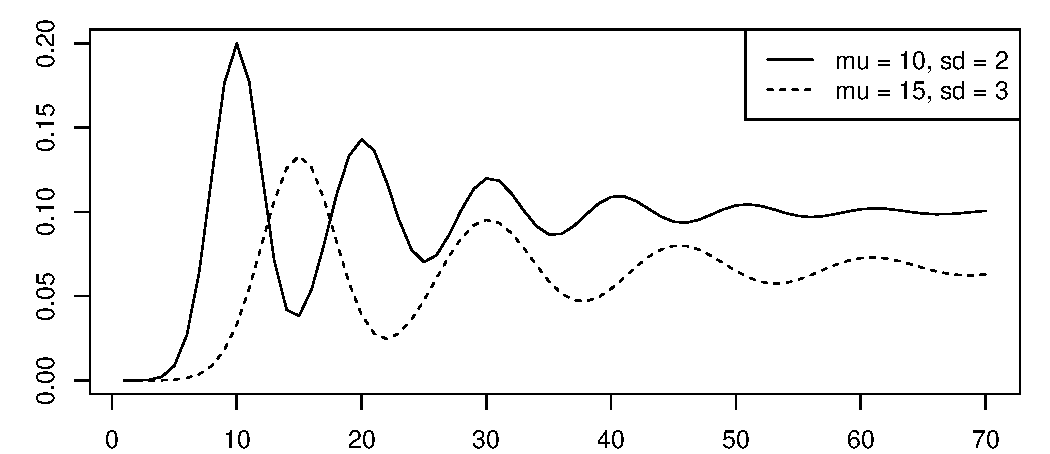
\includegraphics[width=0.40\textwidth]{articles/pics/sdm_paper/pccfExamples.pdf}
\caption{An example of two Gaussian PCCF functions.
}
\label{fig:pccf_example}
\end{figure}
Local extrema of the PCCF function correspond to the time moments $l \mu, l \in \mathbb{Z}$. % where $l$ is a set of positive integers.
PCCF values converge to limits as defined in \Eq{eq:pccf_limit_proof} $L=1/10$ and $L=1/15$.

\subsection{PCCF update after a confirmed change.}
Typically, a detector would have no internal means to know for sure whether $\Event{t}{+}$ is TP or FP.
If we have a feedback mechanism indicating with some time delay $D$ when a change $c_i$ did happen,
we can update PCCF to make our detector more confident about the future change points.
Given a known $c_i$, we recompute PCCF starting from that point.
An updated PCCF is depicted by the dotted line in Figure~\ref{fig:conffunction}.
In Figure~\ref{fig:conffunction} we can see an example of how PCCF oscillates having local maximums at moments $t = k \mu$ until converging to the limit $L=0.1$.
An event at the moment $t=200$ was confirmed as a change and new PCCF is calculated (dashed line).

If we do not reestimate $\theta$ then update procedure is very fast as we simply shift already computed PCCF along the time axis.
\begin{figure}[htb!]
\centering
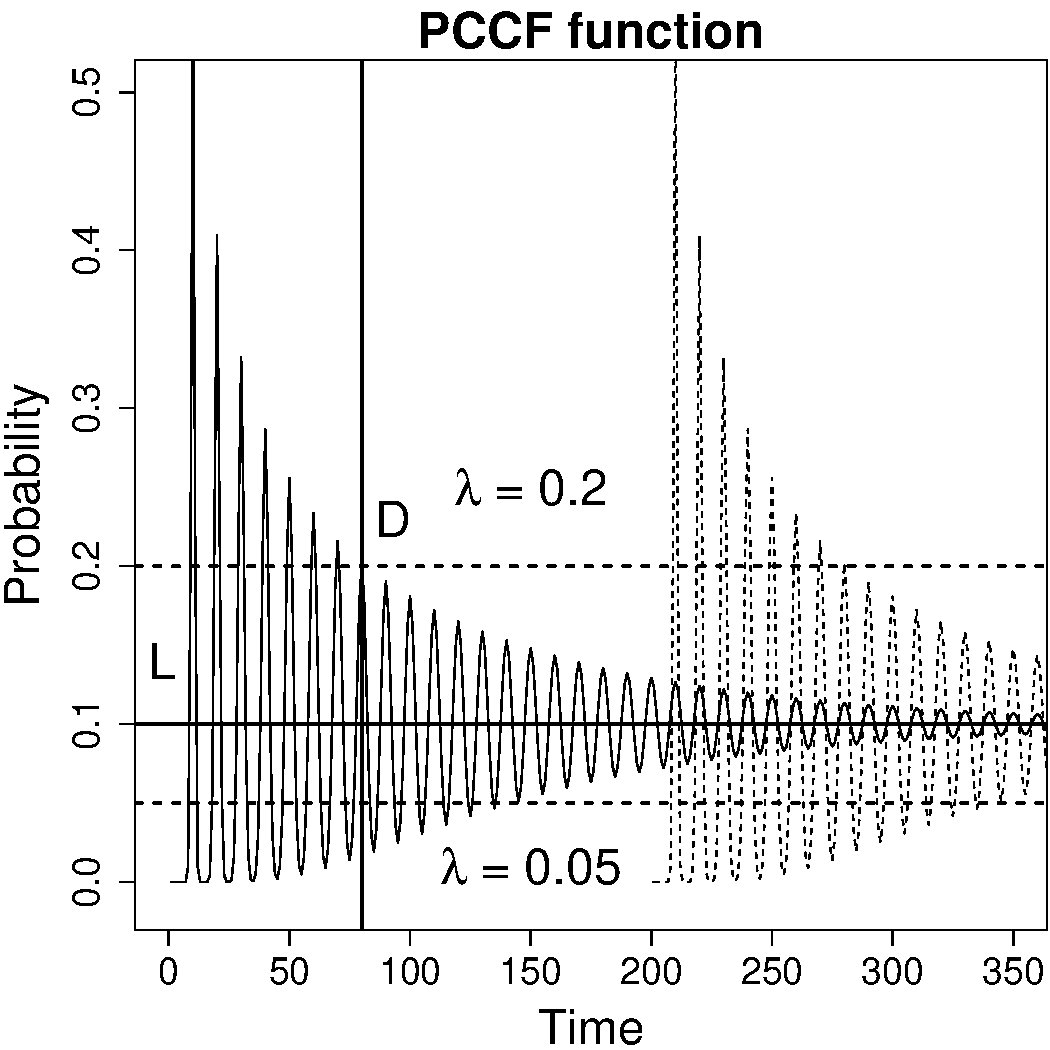
\includegraphics[width=0.35\textwidth]{articles/pics/sdm_paper/PCCF.pdf}
\caption{PCCF converges to the limit $L = 0.1$ depicted by the horizontal bold line.
Two horizontal lines $\lambda$ illustrate possible thresholds above and below the limit.
Vertical line $D$ depicts delay of change confirmation.
}
\label{fig:conffunction}
\end{figure}


\subsection{PCCF pseudo-code}
\label{subsec:pccf_pseudo_code}
In Algorithm~1, in line 11,  a zero-matrix of size $T$ is initialized with the first column filled by initial Pmf values $p(c_1)$.
In line 12 a square lower triangular matrix (Eq.~\ref{eq:second_pccf_matrix}) is generated using the function {\tt WeightsMatrix()}.
Next the probabilities for individual changes in a sequence
$\Collect{ c_i }_{i=1}^k$
are updated within the loop (line 14).
PCCF is calculated in line 15 by summing up probabilities in the columns of matrix $P$.
\begin{algorithm}
    \label{alg:pccfalg}
\begin{algorithmic}[1]
\Function{WeightsMatrix}{T,$\theta$}
    \State M = zeros(T, T);  M[1, :] = 1:T
	\For{i = 2:T}
		\For{j = i:T}
			\State M[i,j] = M[i-1, j-1]
		\EndFor
	\EndFor
	\State \textbf{return} Pmf($M^T$ $| \theta$)
\EndFunction
\\
\Function{PCCF}{$T, \theta=(\mu,\sigma)$}
\State P = zeros(T,T)
\State P[:,1] = Pmf(1:T $| \theta$) \Comment{Pmf fo the first change}
\State W = WeightsMatrix(T,$\theta$)
\For{i = 1:T-1}
	\State P[i+1:T,i+1]=W[1:T-i,1:T-i] * P[i:end-1, i]
\EndFor
\State \textbf{return} sum(P,2) \Comment{Sum of columns}
\EndFunction
\end{algorithmic}
\caption{PCCF function pseudo-code}
\end{algorithm}



\section{From BLPA}

\section{From Journal}

\section{Recurrency}

Adaptive learning in concept drift.
Predictability of events in the data stream.
~\cite{feller2008introduction}
Sums of independent random variables.
Recurrency is a form of predictability.

\subsection{Relevant material from Feller textbook}

The basic theory is as follows~\cite{feller2008introduction}.
In a sequence of Bernoulli trials the waiting time up to the first event gas a geometric distribution.
After the first event the process starts anew, and the number of trials between $n$ and $n+1$ th events has the same geometric distribution.
\begin{definition}
	Let $a_1, a_2, \dots, $ be a sequence of real numbers. If 
	\begin{equation}
		A(s) = a_0 + a_1 s + a_2 s^2 + \dots 
	\end{equation}
    converges in some interval $-s_0 < s < s_0 $ , then $A(s)$ is called the generarating function of the sequence $\{a_j\}$. 
\end{definition}

From\cite{wasserman2013all}
\begin{definition}
	The moment generating function MGF, or Laplace transform, of $X$ is defined by
	\begin{equation}
		\psi_X = \mathbb{E}(e^{tX}) = \int e^{tX} dF(x) 
	\end{equation}
where $t$ varies over the real numbers.
\end{definition}

\subsection{Inter-arrival times modeling}

Basic theory.
\begin{definition}
	A function $\mathbb{P}$ that assigns a real number $\mathbb{P}(A)$ to each event $A$ is a probability distribution if \\
	Axiom 1: $\mathbb{P}(A) \geq 0$ for every $A$\\
	Axiom 2: $\mathbb{P}(\Omega) = 1$\\
	Axiom 3: If $A_1, A_2, \dots $ are disjoint then 
	\begin{equation}
		\mathbb{P} \Big( \bigcup\limits_{i=1}^{\infty} A_i  \Big) = \sum_{i=1}^{\infty} \mathbb{P}(A_i)
	\end{equation}
\end{definition}
Commonly used probability distributions for modelling inter-arrival times.


\section{Pccf}~\label{sec:pccf}

If change points are expected to reoccur in the input signal, then this prior information can be used to approximate prediction time intervals, or regions of interest (ROI), where changes are most likely to appear in the future.
Once calculated, and if predictions are correct, then this information can further be used to reduce the false alarm rate of the change detection process, and potentially to reduce detection delays too.
FA rate can be decreased just by disregarding detections outside prediction intervals, and the detection delay can be decreased by increasing sensitivity of the detector within prediction intervals.
But, as mentioned, if sensitivity is increased, then probability of FA events will also increase.
Possibility of decreasing detection delays in the presence of prediction interval is a subject of Experiments section.
We describe next how to calculate prediction intervals for reoccurring change points.

To calculate ROIs for recurrent change points we use a prediction confidence change function (Pccf) proposed in our previous work~\cite{MaslovSDM2016}, where it was calculated using convolutions.
Below we calculate Pccf for several commonly used distributions of inter-arrival times values using moment generating functions, what is a more concise way than when using convolutions.
Let's start with definitions.
\begin{definition}
	Change points $t_i^{\text{c}}$ are recurrent if their inter-arrival times $t_{i}^{c} - t_{i-1}^{c}$
	% \begin{equation}\label{eq:recurrence_relation}
	%     \Delta_i = t_{i}^{c} - t_{i-1}^{c}
	% \end{equation}
	are i.i.d.\ from the same probability distribution.
	E.g., $t_{i}^{c} - t_{i-1}^{c} \sim \mathbb{N}(\mu, \sigma)$ if $\sigma$ is small.
\end{definition}
%The recurrence relation for recurrent changes is \begin{equation} x_{n+1} = x_n + \delta_n \end{equation}
Pccf function value at time moment $t_i$ is a probability estimator of recurrent change point to occur at this time moment.
%Recurrent changepoints form a sequence determined by recurrence relation given by Equation~\ref{eq:recurrence_relation}.
% $t_{i}^{\text{CHP}} = t_{i-1}^{\text{CHP}} + \Delta_i$.
Pccf can be represented as a matrix~\ref{eq:pccf_matrix} in which elements at row $k$ and column $i$ are probability estimates for change point $t_k^{\text{c}}$ to appear at time moment $t_i$.
\begin{equation}~\label{eq:pccf_matrix}
	\text{PCCF}_{k,i} \equiv P(t_{k}^{\text{c}} = t_i) % \: \forall \:  k, i \in [1,\dots,N
\end{equation}
When calculating ROIs we are interested in total probability of any changepoint occurring at every time moment within prediction horizon.
Since events $t_k^{\text{c}} = t_i$ are disjoint we need to sum up rows of the matrix $\text{PCCF}_{k,i}$
\begin{equation}~\label{eq:pccf_vector}
	\text{PCCF}_{i \in 1:N} = \sum_{k=1}^{N} P(t_k^{\text{c}} = t_i) \equiv \sum_{k=1}^{N} \text{PCCF}_{k,i}
\end{equation}
Further by Pccf we call the vector given by Equation~\ref{eq:pccf_vector}.

The sum~\ref{eq:pccf_vector} can be calculated using the notion of moment generating function (Mgf).
As an example, let's assume a Gaussian distribution for inter-arrival times, i.e. $t_{i}^{\text{c}} - t_{i-1}^{\text{c}} \sim \mathbb{N}(\mu, \sigma)$,
with $\sigma$ small enough so that every next change can not happen before the previous one.
For example, if $\mu=60$ seconds and standard deviation is $\sigma=5$ seconds then, using Chebyshev's inequality~\ref{eq:chebyshev_ineq}, probability of
$\mathbb{P}(|t_{i}^{\text{c}} - t_{i-1}^{\text{c}}| \geq 60) \leq 0.007$.
\begin{equation}\label{eq:chebyshev_ineq}
	\mathbb{P}(|X-\mu| \geq k \sigma) \leq \frac{1}{k^2} % %\mathbb{P}(|X-\mu| \geq t) \leq \frac{\sigma^2}{t^2}
\end{equation}
%\subsec{Predicting sequential events}
% Resources
% \href{https://www.youtube.com/playlist?list=PL2SOU6wwxB0uwwH80KTQ6ht66KWxbzTIo}{Statistics 110: Probability}
%- [lec24] [Lecture 24: Gamma distribution and Poisson process](https://www.youtube.com/watch?v=Qjeswpm0cWY&index=24&list=PL2SOU6wwxB0uwwH80KTQ6ht66KWxbzTIo)
%- [lec22] [Lecture 22: Transformations and Convolutions](https://www.youtube.com/watch?v=yXwPUAIvFyg&list=PL2SOU6wwxB0uwwH80KTQ6ht66KWxbzTIo&index=22)
%- [lec17] [Lecture 17: Moment Generating Functions](https://www.youtube.com/watch?v=N8O6zd6vTZ8&index=17&list=PL2SOU6wwxB0uwwH80KTQ6ht66KWxbzTIo)
%- [lec18] [Lecture 18: Mgfs Continued](https://www.youtube.com/watch?v=tVDdx6xUOcs&list=PL2SOU6wwxB0uwwH80KTQ6ht66KWxbzTIo&index=18)
%- [math.tntech.edu: Sum of independent random variables](http://math.tntech.edu/ISR/Introduction_to_Probability/Distributions_of_Functions/thispage/newnode11.html)
%- [Table of Common Distributions](http://www.stat.tamu.edu/~twehrly/611/distab.pdf) taken from Statistical Inference by Casella and Berger
%The sum~\ref{eq:pccf_sum} can be calculated by calculating Mgf of the sum of i.i.d.\ variables and after that by pattern\ - similarity to the Mgf of individual variable find the PDF of the sum.
%\begin{definition}
By definition, Mgf, or Laplace transform, of random variable $X$ is~\ref{eq:mgf}
%~\footnote{Mgf is $\mathbb{E}(e^{tX})$ while characteristic function is $\mathbb{E}(e^{i t X})$.}
\begin{equation}\label{eq:mgf}
	M_{X}(t) = \mathbb{E}(e^{t X}), \: t \in \mathbb{R}
\end{equation}
%\begin{equation}~\label{eq:mgf}
%	%\psi_{X}(t) = \mathbb{E}(e^{t X}) = \int e^{tX} d F(x)
%	M_{X}(t) = \mathbb{E}(e^{t X})
%\end{equation}
% Moments of a distribution is computed as $\psi^{(k)} (0)=\mathbb{E}(X^k)$.
% Mgfs is a convenient tool to obtain distribution of sums of random variables.
Using the property that expected value of the product of two independent random variables is the product of their expected values $\mathbb{E}(X \dot Y)=\mathbb{E}(X)\mathbb{E}(Y)$, Mgf of the sum of independent random variables is a product of individual Mgfs (Equation~\ref{eq:mgf_of_sum}).
\begin{equation}\label{eq:mgf_of_sum}
	M_{X+Y}(t) = \mathbb{E}(e^{t (X+Y)}) = \mathbb{E}(e^{t X}) \mathbb{E} (e^{t Y}) \equiv M_{X}(t) M_{Y}(t)
\end{equation}
For the Gaussian distribution Mgf is $\exp{(\mu t + \frac{\sigma^2 t^2}{2})}$ and therefore
\begin{equation}\label{eq:mgf_gauss}
	M_{X+Y}^{\text{Gaussian}}(t)  = \exp \Big ((\mu_X + \mu_Y) t + \frac{(\sigma_X^2 + \sigma_Y^2) t^2}{2} \Big )
\end{equation}
But~\ref{eq:mgf_gauss} is Mgf of the Gaussian distribution with parameters $\mu=\mu_1+\mu_2$ and $\sigma=\sqrt{\sigma_X^2 + \sigma_Y^2})$.
Therefore if probability distribution of the first change point is $t_1^{\text{c}} \sim \mathbb{N}(\mu, \sigma)$ then $t_2^{\text{c}} \sim \mathbb{N}(2\mu, \sigma \sqrt{2})$, etc.
And Pccf is a sum~\ref{eq:pccf_gaussian}
\begin{equation}\label{eq:pccf_gaussian}
	\text{PCCF}^{\text{Gaussian}} \equiv \sum_{k=1}^N \mathbb{N}(k \mu, \sqrt{k} \sigma)
\end{equation}

Using the same logic it is straightforward to calculate Pccfs for Exponential and Gamma distributions (Table~\ref{table:pccfs}).
\begin{table}[!htb] \caption{Pdf's for distributions of inter-arrival times.}\label{table:pccfs}
	\begin{center}
		\begin{tabular}{|l|l|c|c|}
			\hline
			Distribution & Mgf & PDF of the $k$-th event & PCCF  \\[5pt]
			\hline
			Gaussian & $\exp{ (\mu t + \frac{\sigma^2 t^2}{2}) }$ & $\mathcal{N}(k \mu, \sqrt{k} \sigma)$ & $\sum_{k=1}^N \mathcal{N}(k \mu, \sqrt{k} \sigma)$ \\
			Gamma $\Gamma(\alpha, \lambda)$ & $\Big ( \frac{1}{1- \lambda t} \Big )^{\alpha}$ & $\Gamma(k \alpha, \lambda)$ & $\sum_{k=1}^N \Gamma(k \alpha, \lambda)$\\
			Exponential & $\frac{\lambda}{\lambda - t}$ & $\Gamma(k, \lambda)$ & $\sum_{k=1}^N \Gamma(k, \lambda)$\\
			\hline
		\end{tabular}
	\end{center}
\end{table}
Figure~\ref{fig:pccf_example} depicts Gaussian Pccf.
Prediction intervals (ROI) can be calculated by applying a threshold value for Pccf and then ROIs will be determined by time moments when Pccf exceeds this threshold.
In this way we would take into account uncertainty in the predictions for $k$-th change points which will increase as $\sqrt{k} \sigma$ (Equation~\ref{eq:pccf_gaussian}).
Another way is to use the property that Pccf extremums are equally spaced (Equation~\ref{eq:rois})~\cite{MaslovSDM2016} by time intervals $\mu$.
After estimating $\mu$ between changes and choosing the number of change points $k$ to predict and ROIs width prediction interval are determined by Equation~\ref{eq:rois}.
\begin{equation}\label{eq:rois}
	\text{ROI}s = (\mu \pm \text{ROI}_{\text{Width}}, 2 \mu \pm \text{ROI}_{\text{Width}}, \dots , k \mu \pm \text{ROI}_{\text{Width}}).
\end{equation}
\begin{figure}[!htb]
	\centering
	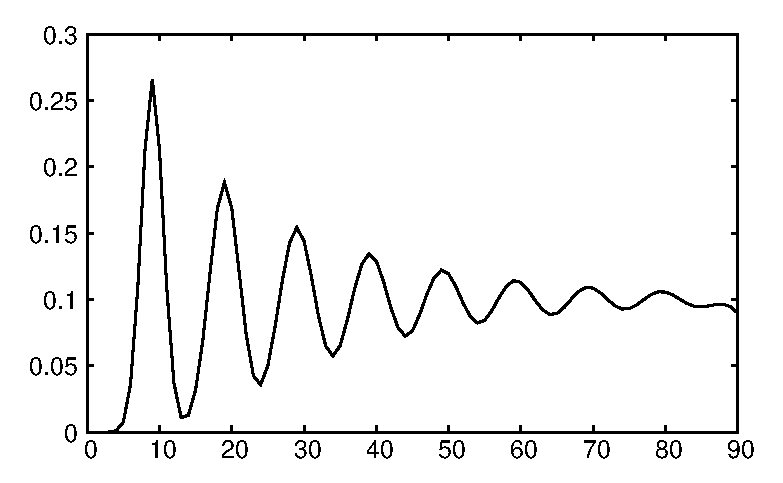
\includegraphics[width=0.7\textwidth]{images/example_pccf.eps}
	\caption{Pccf example}\label{fig:pccf_example}
\end{figure}


\section{Integration with Bayesian detector}


\section{Integration with CuSum}


%~\footnote{we useterms recurrent and reoccurring interchangebly}
% The difference to the previous work is that we calculate Pccf in a concise
% way using moment generating functions and we calculate it for several
% commonly used distributions used for inter arrival time modelling.
%In our previous work we applied threshold value to the calculated probability estimates, but now we found it much more practical just to use equally spaced time moments surrounded by time intervals of a fixed size.
% Probability estimates given by Pccf should be used to assess confidence intervals for predictions and for assessment of how many changes in the future we want to make a prediction for.

% Mgfs for commonly used for inter-arrival times modelling distributions are~\cite{wasserman2013all}
% as follows.
% for Exponential distribution with rate $\lambda$ it is $\frac{\lambda}{\lambda - t}$;
% and for the Gamma distribution $\Gamma(\alpha, \lambda)$ is $\Big ( \frac{1}{1- \lambda t} \Big )^{\alpha}$.
% $\Big (\frac{\lambda}{\lambda - t} \Big)^{\alpha}$ %([ref](http://math.tntech.edu/ISR/Introduction_to_Probability/Distributions_of_Functions/thispage/newnode11.html))
%
% % POSISSON is not needed, as we model inter-arrival times, not number of occurences
%\item Poisson is $e^{\lambda (e^t-1)}$
%
% $\mathbb{E}(e^{tX}) = \sum_{k=0}^{\infty} e^{tk} e^{-\lambda} \lambda^k/k! = e^{\lambda (e^t-1)}$
% https://en.wikipedia.org/wiki/Gamma_distribution#Summation
% https://stats.stackexchange.com/questions/51605/the-sum-of-two-independent-gamma-random-variables
% proof: https://en.wikipedia.org/wiki/Characteristic_function_%28probability_theory%29#Example
%Proof for the Gamma can be found \href{https://en.wikipedia.org/wiki/Characteristic\_function\_\%28probability\_theory\%29#Example}{here}. Characteristic functions are $\phi_X(t)=(1-\lambda i t)^{-a}$ and $\phi_Y(t)=(1-\lambda i t)^{-b}$. Therefore $\phi_{X+Y}(t) = (1-\lambda i t)^{-(a+b)}$.
%
% Poisson & $\mathbb{E}(e^{tX}) = \sum_{k=0}^{\infty} e^{tk} e^{-\lambda} \lambda^k/k! = e^{\lambda (e^t-1)}$ & Inter-arr. times are from Exp. And Pdf is for Gamma \\
%Weibull? & & p pp\\
% Gamma~\cite{wasserman2013all}
%
%  Corresponding Mgfs for the sums are as follows.
%  for Gamma distribution $M_{X+Y} (t) =  \Big (\frac{\lambda}{\lambda - t} \Big)^{a + b}$
%  and for Exponential distribution is $\frac{\lambda}{\lambda-t}$.
%
%  Gaussian,
%  If $X \sim N(\mu_X, \sigma_X)$ and $Y \sim N(\mu_Y,\sigma_Y)$ then $X+Y \sim N(\mu_X + \mu_Y, \sqrt{\sigma_X + \sigma_Y})$
%  $$M_{X+Y}(t) = \exp \Big ( t \mu_X  + \frac{\sigma_X^2 t^2}{2} \Big) \cdot \exp \Big ( t \mu_Y  + \frac{\sigma_Y^2 t^2}{2} \Big) = \exp \Big [ (\mu_X + \mu_Y) t + \frac{(\sigma_X^2 + \sigma_Y^2) t^2}{2} \Big ] $$ which is a characteristic function of the normal distribution with parameters $\mu =  \mu_X + \mu_Y$ and $ \sigma^2 = \sigma_X^2 + \sigma_Y^2$.
%
%
% $\Gamma(k, \lambda)$.
% Copied to for)thesis.tex
%
%\begin{itemize}
%	% POSISSON is not needed, as we model inter-arrival times, not number of occurences
%	%    %\item \textbf{For the Poisson.}
%	%$$M^P_{X+Y} (t) =  e^{\lambda (e^t-1)}  e^{\mu (e^t-1)} =  e^{(\lambda+\mu) (e^t-1)}$$
%	%It means $X+Y \sim \text{Poiss}(\lambda + \mu)$ (note: the sum of two Poissons is also a Poisson, which is not general for any distribution)
%	\item \textbf{Gaussian}
%	If $X \sim N(\mu_X, \sigma_X)$ and $Y \sim N(\mu_Y,\sigma_Y)$ then $X+Y \sim N(\mu_X + \mu_Y, \sqrt{\sigma_X + \sigma_Y})$
%	$$M_{X+Y}(t) = \exp \Big ( t \mu_X  + \frac{\sigma_X^2 t^2}{2} \Big) \cdot \exp \Big ( t \mu_Y  + \frac{\sigma_Y^2 t^2}{2} \Big) = \exp \Big [ (\mu_X + \mu_Y) t + \frac{(\sigma_X^2 + \sigma_Y^2) t^2}{2} \Big ] $$
%
%	which is a characteristic function of the normal distribution with parameters $(\mu =  \mu_X + \mu_Y, \sigma^2 = \sigma_X^2 + \sigma_Y^2)$.
%
%	\item \textbf{Gamma}
%	If $X \sim \Gamma(a, \lambda), Y \sim \Gamma(b, \lambda)$ then $X+Y \sim \Gamma(a+b, \lambda)$.
%
%	$$M_{X+Y} (t) = M_X (t) \cdot M_Y (t) = \Big (\frac{\lambda}{\lambda - t} \Big)^{a}  \Big (\frac{\lambda}{\lambda - t} \Big)^{b} =  \Big (\frac{\lambda}{\lambda - t} \Big)^{a + b}$$
%
%	\item \textbf{Exponential}
%	Mgf for the exponential distribution with $\lambda=1$ is $\frac{1}{1-t}$ where $t<1$.
%	% Lec.14 (Statistics 101): https://www.youtube.com/watch?v=Qjeswpm0cWY&index=24&list=PL2SOU6wwxB0uwwH80KTQ6ht66KWxbzTIo
%	% START: 23:27
%	% Using the property of moment generating functions (by definition)
%	% \[\psi_{X+Y}(t) = \mathbb{E}(e^{t (X+Y)}) = \mathbb{E}(e^{t X}) \mathbb{E} (e^{t Y})\]
%	Mgf for the $n$-th event $T_n = \sum_{j=1}^{n} X_j, \text{ where } X_j \sim e^{-\lambda t}$ is $\Big ( \frac{1}{1-t} \Big )^n$.
%	But Mgf for $Y \sim \Gamma(n,1)$ is also $\Big(\frac{1}{1-t} \Big)^n$.
%	Therefore if inter-arrival times are i.i.d. from the exponential distribution with parameter $\lambda$ the PDF for the k-th event is $\Gamma(k, \lambda)$.
%	%\begin{equation}
%	%    \mathbb{E}(e^{tY}) = \frac{1}{\Gamma(n)} \int_{0}^{\infty} e^{ty} y^{n} e^{-y} \frac{d y}{y} = \frac{1}{\Gamma(n)} \int_{0}^{\infty} y^n e^{-(1-t)y} \frac{d y}{y}
%	%\end{equation}
%	%Let, $x=(1-t)y$, then $d x = (1-t) d y$, then we get
%	%\begin{equation}
%	%    \mathbb{E}(e^{tY}) = \frac{(1-t)^{-n}}{\Gamma(n)} \int_{0}^{\infty} x^n e^{-x} \frac{d x}{x} = \Big(\frac{1}{1-t} \Big)^n
%	%    \label{eq:mgf_gamma_1}
%	%\end{equation}
%	%This is (Equation~\ref{eq:mgf_gamma_1}) the same Mgf as Mgf for the sum of i.i.d. from Exponential distribution with $\lambda=1$ (Equation~\ref{eq:mgf_exp_n}).
%
%	%If $X \sim Exp(\lambda_1)$ and $Y \sim Exp(\lambda_2)$ then $X+Y \sim $
%	%$$M^E_{X+Y}(t) = \frac{\lambda_1}{\lambda_1 - t} \frac{\lambda_2}{\lambda_2 - t}$$
%\end{itemize}


%, i.e.  $\sum_{k=1}^{N} P(t_k^{\text{CHP}} = t_i)$.
%	\begin{equation}
%		\text{Any } t_{k}^{\text{CHP}} = t_i
%		% \text{ or } t_{2}^{\text{CHP}} = t   \dots t_{k}^{\text{CHP}} = t
%		%C_1 = t \text{ or } C_2 = t \text{ or } \dots C_n = t
%		\label{eq:events_union}
%	\end{equation}
%Since events $t_k^{\text{CHP}} = t_i$ are disjoint Pccf can be calculated as
%\begin{equation}
%	\sum_{i=1}^{N} \sum_{k=1}^{N} P(t_k^{\text{CHP}} = t_i).
%\end{equation}
%\begin{equation}
%	P\Big(\bigcup\limits_{k=1}^{N} (t_k^{\text{CHP}} = t_i) \Big ) = \sum_{k=1}^{N} P(t_k^{\text{CHP}} = t_i)
%\end{equation} % Wasserman, page5

